%!TEX output_directory = aux

\documentclass[11pt]{article}

\usepackage[english]{babel}

% ---- FONT & MICROTYPOGRAPHY ----
\usepackage[utf8]{inputenc}
\usepackage[T1]{fontenc}
\usepackage{microtype}
\usepackage{moresize}

% ---- FORMATTING ----
\usepackage{csquotes,textcase,xspace}

% ---- PAGE LAYOUT ----
\usepackage{geometry}
\geometry{top=2.5cm,bottom=2cm,inner=2cm,outer=2cm,footnotesep=7mm plus 4pt minus 4pt}
\usepackage{setspace}
\setstretch{1.1}

% ---- GRAPHIQUE ----
\usepackage{graphicx}
\usepackage{xcolor}
\usepackage[font=small,labelfont=bf,labelsep=space]{caption}
\usepackage{subfigure}
\captionsetup{width=0.9\textwidth,font={small,stretch=1.1}}
\addto\captionsenglish{\renewcommand{\figurename}{Fig.}}
\addto\captionsenglish{\renewcommand{\tablename}{Tab.}}
\definecolor{JoliBleu}{rgb}{0,0.55,0.55}
\definecolor{JoliVert}{rgb}{0.15,0.6,0}
\definecolor{JoliRouge}{rgb}{0.86,0.08,0}
\definecolor{JoliJaune}{rgb}{1,0.75,0}
\definecolor{JoliGris}{rgb}{0.52,0.52,0.51}
\definecolor{myblue}{RGB}{26, 77, 116}
\definecolor{myorange}{RGB}{181, 116, 30}
\definecolor{mydarkorange}{RGB}{166, 88, 0}
\definecolor{mygreen}{RGB}{21, 124, 80}
\definecolor{myblack}{RGB}{43, 65, 82}
\definecolor{myred}{rgb}{0.5, 0.0, 0.13}

% ---- SECTIONING ----
\usepackage{titlesec}
\titleformat{\section}[block]{\Large\boldmath\bfseries}{\thesection}{1em}{}
\titleformat{\subsection}[block]{\large\boldmath\bfseries}{\thesubsection}{0.5em}{}
\usepackage{appendix}
\renewcommand{\setthesection}{\Alph{section}}
\renewcommand{\restoreapp}{}
\makeatletter
\renewcommand{\theequation}{\thesection.\arabic{equation}}
\@addtoreset{equation}{section}
\makeatother

% ---- FOOTERS HEADERS ----
\usepackage[bottom]{footmisc}
\usepackage{fancyhdr}

% ---- TABLE OF CONTENTS ----
\usepackage{titletoc}
\setcounter{tocdepth}{3}

% ---- BIBLIOGRAPHY ----
\usepackage[nosort]{cite}
\bibliographystyle{utphys}
\newcommand{\eprint}[1]{{\href{http://arxiv.org/abs/#1}{\texttt{[#1]}}}}
\newcommand{\eprintN}[1]{{\href{http://arxiv.org/abs/#1}{\texttt{#1 [hep-th]}}}}
\newcommand{\doi}[2]{\href{http://dx.doi.org/#2}{#1}}

% ---- HYPER REF ----
\usepackage{hyperref}
\hypersetup{colorlinks=true,
        pdfstartview=FitV,
        linkcolor= mydarkorange,
        citecolor= mydarkorange,
        urlcolor= JoliGris!60!black,
        hypertexnames=false,
        linktoc=page}

% ---- TIKZ ----
\usepackage{tikz}
\usetikzlibrary{calc}

% ---- MATHS ----
\usepackage{amsmath,amssymb,amsfonts,dsfont}
\usepackage{mathrsfs}
\usepackage{physics}
\usepackage{ytableau}
\ytableausetup{boxsize=1.1em,centertableaux}
\usepackage{stmaryrd}
\usepackage{nicefrac}
\allowdisplaybreaks[1]
% \usepackage{bbold}
\usepackage{cases}
\usepackage{bm}
\usepackage{extarrows}

% ---- TABLES ----
\usepackage{multirow}
\usepackage{booktabs}
\usepackage{pdflscape}
\usepackage{array}

% ---- ENUMERATION ----
\usepackage[shortlabels]{enumitem}

% ---- MATHS COMMANDS ----
\newcommand{\A}{\ensuremath{\mathcal{A}}\xspace}
\newcommand{\F}{\ensuremath{\mathcal{F}}\xspace}
\renewcommand{\H}{\ensuremath{\mathcal{H}}\xspace}
\newcommand{\M}{\ensuremath{\mathcal{M}}\xspace}
\renewcommand{\P}{\ensuremath{\mathcal{P}}\xspace}
\newcommand{\J}{\ensuremath{\mathcal{J}}\xspace}
\renewcommand{\d}{\ensuremath{\mathrm{d}}\xspace}
\renewcommand{\H}{\ensuremath{\mathcal{H}}\xspace}
\newcommand{\SO}{\ensuremath{\mathrm{SO}}\xspace}
\renewcommand{\O}{\ensuremath{\mathrm{O}}\xspace}
\newcommand{\SL}{\ensuremath{\mathrm{SL}}\xspace}
\newcommand{\E}{\ensuremath{\mathrm{E}}\xspace}
\newcommand{\R}{\ensuremath{\mathbb{R}}\xspace}
\newcommand{\Odd}{\ensuremath{\mathrm{O}(d,d)}\xspace}
\newcommand{\odd}{\ensuremath{\mathfrak{o}(d,d)}\xspace}
\renewcommand{\Tr}[1]{\ensuremath{\mathrm{Tr}\left(#1\right)}\xspace}

\newcommand{\be}{\begin{equation}}
\newcommand{\ee}{\end{equation}}

% ---- COMMENTS ----
\newcommand{\ce}[1]{\marginpar{\parbox{\marginparwidth}{\boldmath $\Longleftarrow$}}
{\boldmath\bfseries (ce: #1)}}

% ---- TITLE PAGE ----
\usepackage[affil-it]{authblk}
\def\preprint{}

\makeatletter
\def\@maketitle{%
  \newpage
  \null\hfill\texttt{\preprint}
  \vskip 4em%
  \begin{center}%
  \let \footnote \thanks
    {\LARGE\bfseries\boldmath \@title \par}%
    \vskip 2.5em%
    % {\large
    %   \lineskip .5em%
    %   \begin{center}
    %     \begin{minipage}{0.95\textwidth}
    %         \begin{tabular}[t]{c}%
    %         \@author
    %         \end{tabular}
    %     \end{minipage}    
    %   \end{center}\par}%
    % \vskip 1em%
   {\large \@date}%
  \end{center}%
  \par
  \vskip 1.5em}
\makeatother

\renewcommand\Authands{ and }

\title{Notes: New gaugings in 3d from three-form}
\author{}

\begin{document}

\maketitle

Three-form field-strengths are auxiliary in three dimensions and can be integrated out, giving rise to additional gaugings and contributions to the scalar potential, or equivalently leading to new terms in the embedding tensor (see ref.~\cite{Deger:2014ofa,Eloy:2021fhc} for explicit realisations in half-maximal supergravity). We want to generalize this to maximal supergravity. For a given $\E_{8(8)}$ consistent truncations of gauge group $G_{0}$, we ask the question whether it is possible to turn on additional components in the embedding tensor (corresponding to three-form degrees of freedom). If so, the new consistent truncation has gauging $G\supset G_{0}$. We first need to identify which components of the embedding tensor correspond to these degrees of freedom, and to count the number of singlets under $G_{0}$ within them. There will be at least one singlet, corresponding to the gauging of $G_{0}$ in the initial truncation. (\ce{What if the original truncation uses components of the embedding tensor not related to three-forms?}) Any additional singlet would indicate additional parameters to play with, possibly leading to new vacua.

\section{\texorpdfstring{${\rm AdS}_{3}\times S^{3}$}{AdS3xS3}: a proof of concept}
We start by reproducing the analysis of ref.~\cite{Eloy:2021fhc} to prove the validity of our method. They are two different half-maximal supergravities in six dimensions, with ${\cal N}=(2,0)$ and ${\cal N}=(1,1)$. They both admit consistent truncation on $S^{3}$~\cite{Hohm:2017wtr,Samtleben:2019zrh}, leading to half-maximal gauged supergravity in three dimensions with duality group $\SO(8,4)$. These truncations have isometry group $\SO(4)\times\SO(4)$ and are constructed in terms of two different $\SO(3,3)$ subgroups of $\SO(8,4)$:
\begin{subequations}
  \begin{align}
    {\cal N}=(2,0):&\qquad \SO(8,4)\longrightarrow\SO(3,3)_{(2,0)}\times \SO(5,1)\longrightarrow\SO(3,3)_{(2,0)}\times \SO(5), \label{eq:SO84decomp20}\\
    {\cal N}=(1,1):&\qquad \SO(8,4)\longrightarrow\SO(4,4)\times \SO(4)\longrightarrow\SO(3,3)_{(1,1)}\times\R_{+}\times\SO(4). \label{eq:SO84decomp11}
  \end{align}
\end{subequations}

  \subsection{\texorpdfstring{${\cal N}=(2,0)$}{N=(2,0)} six-dimensional supergravity}

  \paragraph{6d origin of the three-forms} The ${\cal N}=(2,0)$ supergravity features 5 self-dual two-forms $\hat{B}_{\hat\mu\hat\nu}^{i}$ ($i\in\llbracket1,5\rrbracket$ is the $\SO(5)$ vector index). They lead to two-form potentials $B_{(2)}^{i}$ in 3d, with three-form field strengths dual to purely internal three-form field-strengths $H_{(3)}^{i}$.

  \ce{Should we consider the anti-self dual two-form also?}

  \paragraph{\boldmath $B_{(2)}^{i}$ in $\SO(3,3)_{(2,0)}\times\SO(5)$}
  The coordinates $X^{[MN]}$ of the $\SO(8,4)$ exceptional field theory of ref.~\cite{Hohm:2017wtr} sit in the adjoint $\bm{66}$ of $\SO(8,4)$. Under eq.~\eqref{eq:SO84decomp20}, it decomposes into
  \begin{equation}  
    \bm{66} \longrightarrow (\bm{6},\bm{1}) \oplus (\bm{6},\bm{5}) \oplus (\bm{15},\bm{1}) \oplus (\bm{1},\bm{5}) \oplus (\bm{1},\bm{10}).
  \end{equation}
  Further decomposing $\SO(3,3)_{(2,0)}\times\SO(5)\rightarrow\SL(3)\times\R_{+}\times\SO(5)$, we get
  \begin{equation}
    \begin{aligned}
      \bm{66} &\longrightarrow [(\bm{\bar{3}}_{2},\bm{1})\oplus(\bm{3}_{-2},\bm{1})] \oplus [(\bm{3}_{-2},\bm{5})\oplus(\bm{\bar{3}}_{2},\bm{5})] \oplus [(\bm{3}_{4},\bm{1})\oplus(\bm{1}_{0},\bm{1})\oplus(\bm{8}_{0},\bm{1})\oplus(\bm{\bar{3}}_{-4},\bm{1})] \\
      & \qquad \oplus (\bm{1}_{0},\bm{5}) \oplus (\bm{1}_{0},\bm{10}).
    \end{aligned}
  \end{equation}
  The internal coordinates $y^{m}$ then sit in the representation $(\bm{3}_{4},\bm{1})$ and the two-form potentials $B_{(2)}^{i}$ in $(\bm{3}_{-2},\bm{5})$, they thus originate from the $\SO(3,3)_{(2,0)}\times\SO(5)$ representations $(\bm{15},\bm{1})$ and $(\bm{6},\bm{5})$, respectively.

  \paragraph{\boldmath $H_{(3)}^{i}$ in $\SO(3,3)_{(2,0)}\times\SO(5)$}
  \begin{equation}
    H_{(3)}^{i} \subset(\bm{15},\bm{1})\otimes(\bm{6},\bm{5})=(\bm{6},\bm{5})\oplus(\bm{10},\bm{5})\oplus(\bm{\bar{10}},\bm{5})\oplus(\bm{64},\bm{5}).
  \end{equation}

  \paragraph{\boldmath $H_{(3)}^{i}$ in the embedding tensor}
  The embedding tensor of the $\SO(8,4)$ exceptional theory has two different components: $\theta_{(MN)}\subset\bm{77}$ and $\theta_{[MNPQ]}\subset\bm{495}$. It decomposes as follows under $\SO(8,4)\rightarrow\SO(3,3)_{(2,0)}\times \SO(5)$:
  \begin{equation}
    \begin{aligned}
      \bm{77} &\longrightarrow 2\times(\bm{1},\bm{1}) \oplus (\bm{6},\bm{1}) \oplus {\color{mydarkorange}(\bm{6},\bm{5})} \oplus (\bm{20'},\bm{1}) \oplus (\bm{1},\bm{5}) \oplus (\bm{1},\bm{14}),\\
      \bm{495} &\longrightarrow (\bm{10},\bm{1}) \oplus {\color{mydarkorange}(\bm{10},\bm{5})} \oplus (\bm{\bar{10}},\bm{1}) \oplus {\color{mydarkorange}(\bm{\bar{10}},\bm{5})} \oplus (\bm{15},\bm{1}) \oplus (\bm{1},\bm{5}) \oplus (\bm{1},\bm{10}) \\
      &\qquad\oplus (\bm{6},\bm{10}) \oplus (\bm{6},\bm{\bar{10}}) \oplus (\bm{15},\bm{5}) \oplus (\bm{15},\bm{10}),
    \end{aligned}
  \end{equation}
  where the colored representations are those coming from the three-forms. Only $(\bm{10},\bm{5})$ and $(\bm{\bar{10}},\bm{5})$ feature singlets under the isometry group $\SO(4)\times\SO(4)$. One of these support the $S^{3}$ reduction, while the other can be turned on, leading to new solutions as first demonstrated in ref.~\cite{Hohm:2017wtr,Samtleben:2019zrh}. All singlets sit in $\theta_{MNPQ}$.


 \subsection{\texorpdfstring{${\cal N}=(1,1)$}{N=(1,1)} six-dimensional supergravity}

  \paragraph{6d origin of the three-forms} The ${\cal N}=(1,1)$ supergravity features a two-form $\hat{B}_{\hat\mu\hat\nu}$ Both $\hat{B}_{\hat\mu\hat\nu}$ and its dual lead to two-form potentials in 3d. Their three-form field strengths are dual to purely internal three-form field-strengths $H_{(3)}$ and $*H_{(3)}$, of two-form potentials $C_{(2)}^{1}$ and $C_{(2)}^{2}$.

  \paragraph{\boldmath $C_{(2)}^{1}$ and $C_{(2)}^{2}$in $\SO(4,4)\times\SO(4)$}
  Under $\SO(8,4)\longrightarrow\SO(4,4)\times \SO(4)$, the coordinates $X^{[MN]}$ decompose into
  \begin{equation}  
    \bm{66} \longrightarrow \bm{1}^{(\bm{3},\bm{1})} \oplus \bm{1}^{(\bm{1},\bm{3})} \oplus \bm{8_{\rm v}}^{(\bm{2},\bm{2})} \oplus \bm{28}^{(\bm{1},\bm{1})}.
  \end{equation}
  The internal coordinates and the two-form potentials are singlets under the $\SO(4)$ factor, which is related the 6d vectors only. They thus all belong to the representation $\bm{28}^{(\bm{1},\bm{1})}$.

  \paragraph{\boldmath $H_{(3)}$ and $*H_{(3)}$ in $\SO(4,4)\times\SO(4)$}
  \begin{equation}
    H_{(3)}, *H_{3}\subset\bm{28}^{(\bm{1},\bm{1})}\otimes\bm{28}^{(\bm{1},\bm{1})}=\bm{1}^{(\bm{1},\bm{1})}\oplus\bm{28}^{(\bm{1},\bm{1})}\oplus\bm{35_{\rm v}}^{(\bm{1},\bm{1})}\oplus\bm{35_{\rm s}}^{(\bm{1},\bm{1})}\oplus\bm{35_{\rm c}}^{(\bm{1},\bm{1})}\oplus\bm{300}^{(\bm{1},\bm{1})}\oplus\bm{350}^{(\bm{1},\bm{1})}.
  \end{equation}

  \paragraph{\boldmath $H_{(3)}$ and $*H_{(3)}$ in the embedding tensor}
  \begin{equation}
    \begin{aligned}
      \bm{77} &\longrightarrow {\color{mydarkorange}\bm{1}^{(\bm{1},\bm{1})}} \oplus \bm{1}^{(\bm{3},\bm{3})} \oplus \bm{8_{\rm v}}^{(\bm{2},\bm{2})} \oplus {\color{mydarkorange}\bm{35_{\rm v}}^{(\bm{1},\bm{1})}},\\
      \bm{495} &\longrightarrow {\color{mydarkorange}\bm{1}^{(\bm{1},\bm{1})}} \oplus \bm{8_{\rm v}}^{(\bm{2},\bm{2})} \oplus \bm{28}^{(\bm{1},\bm{3})} \oplus \bm{28}^{(\bm{3},\bm{1})} \oplus {\color{mydarkorange}\bm{35_{\rm s}}^{(\bm{1},\bm{1})}} \oplus {\color{mydarkorange}\bm{35_{\rm c}}^{(\bm{1},\bm{1})}} \oplus \bm{56_{\rm v}}^{(\bm{2},\bm{2})}.
    \end{aligned}
  \end{equation}
  The singlets certainly gauge the trombone symmetry. Each $\bm{35}$ feature $\SO(4)\times\SO(4)$ singlets, but \ce{less clear how to precisely relate to ref.~\cite{Eloy:2021fhc}. Need to consider quadratic constraint?}

  


\section{Truncations within \texorpdfstring{$\SL(8)_{\rm IIB}\subset\E_{8(8)}$}{SL(8)IIB in E8(8)}}
We analyse here whether the type IIB $S^{7}$ truncation of ref.~\cite{Galli:2022idq} admit additional gaugings.

\paragraph{10d origin of the three-forms} Both the 10d two-forms $\hat{C}_{\hat\mu\hat\nu}^{\alpha}$ ($\alpha\in{1,2}$ for $\SL(2)$ doublet) and the 10d four-form $\hat{C}_{\hat\mu\hat\nu\hat\rho\hat\sigma}$ give two-form potentials $C^{\alpha}_{\mu\nu}$ and $C_{\mu\nu mn}$ in 3d ($m,n\in\llbracket1,7\rrbracket$ are $\SL(7)$ indices). Their three-form field-strengths are dual to purely internal seven-form and five-form field-strengths $H_{(7)}^{\alpha}$ and $H_{(5)}$, respectively. We note $C_{(6)}^{\alpha}$ and $C_{(4)}$ the six-form and four-form potentials from which they derive.


\paragraph{\boldmath $C_{(6)}^{\alpha}$ and $C_{(4)}$ in $\SL(8)_{\rm IIB}\times\R_{+}$} In the $\E_{8(8)}\rightarrow\SL(7)\times\SL(2)\times\R_{+}$ decomposition
\begin{equation}
  \begin{aligned}
    \bm{248} \longrightarrow & \ (\bm{7},\bm{1})_{12} \oplus (\bm{\bar{7}},\bm{2})_{9} \oplus (\bm{\bar{35}},\bm{1})_{6} \oplus (\bm{21},\bm{2})_{3} \oplus (\bm{1},\bm{1})_{0} \oplus (\bm{1},\bm{3})_{0} \oplus (\bm{48},\bm{1})_{0} \\
    & \oplus (\bm{\bar{21}},\bm{2})_{-3} \oplus (\bm{35},\bm{1})_{-6} \oplus (\bm{7},\bm{2})_{-9} \oplus (\bm{\bar{7}},\bm{1})_{-12}
  \end{aligned} 
\end{equation}
of the $\E_{8(8)}$ coordinates $X^{M}$, $C_{(6)}^{\alpha}$ and $C_{(4)}$ sit in the representations $(\bm{7},\bm{2})_{-9}$ and $(\bm{35},\bm{1})_{-6}$, respectively.\footnote{The internal coordinates $y^{m}$ are in the representation $(\bm{7},\bm{1})_{12}$, and $\bm{\bar{7}}^{\wedge 4}=\bm{35}$ and $\bm{\bar{7}}^{\wedge 6}=\bm{7}$.} They originate from the representations $\bm{8}_{3}\oplus\bm{63}_{0}$ and $\bm{56}_{1}$ in $\E_{8(8)}\rightarrow\SL(9)\rightarrow\SL(8)_{\rm IIB}\times\R_{+}$ decomposition
\begin{equation}
  \bm{248} \longrightarrow \bm{80} \oplus \bm{84} \oplus \bm{\bar{84}} \longrightarrow \left[\bm{8}_{3} \oplus \bm{1}_{0} \oplus \bm{63}_{0} \oplus \bm{\bar{8}}_{-3}\right] \oplus \left[\bm{56}_{1} \oplus \bm{28}_{-2}\right] \oplus \left[\bm{\bar{28}}_{2} \oplus \bm{\bar{56}}_{-1}\right],
\end{equation}
whereas the internal coordinates are in the representation $\bm{\bar{28}}_{2}$.

\ce{Give further details?}

\paragraph{\boldmath $H_{(7)}^{\alpha}$ and $H_{(5)}$ in $\SL(8)_{\rm IIB}\times\R_{+}$} Now that we know what are the $\SL(8)_{\rm IIB}\times\R_{+}$ representations corresponding to the internal coordinates, $C_{(6)}^{\alpha}$ and $C_{(4)}$, we can infer those of $H_{(7)}^{\alpha}$ and $H_{(5)}$:
\begin{equation}  \label{eq:H7H5inIIB}
  \begin{aligned}
    H_{(7)}^{\alpha} & \subset \bm{\bar{28}}_{2} \otimes \left(\bm{8}_{3}\oplus\bm{63}_{0}\right) = \bm{\bar{8}}_{5} \oplus \bm{\bar{216}}_{5} \oplus \bm{\bar{28}}_{2} \oplus \bm{\bar{36}}_{2} \oplus \bm{\bar{420}}_{2} \oplus \bm{\bar{1280}}_{2}, \\
    H_{(5)} & \subset \bm{\bar{28}}_{2} \otimes \bm{56}_{1} = \bm{8}_{3} \oplus \bm{216}_{3} \oplus \bm{1344}_{3}.
  \end{aligned}
\end{equation}

\paragraph{\boldmath $H_{(7)}^{\alpha}$ and $H_{(5)}$ in the embedding tensor} Under $\E_{8(8)}\rightarrow\SL(9)\rightarrow\SL(8)_{\rm IIB}\times\R_{+}$, the $\E_{8(8)}$ embedding tensor decomposes as
\begin{equation}
  \begin{aligned}
    \bm{3875} &\longrightarrow {\color{mydarkorange}\bm{80}} \oplus \bm{240} \oplus {\color{mydarkorange}\bm{\bar{240}}} \oplus \bm{1050} \oplus {\color{mydarkorange}\bm{\bar{1050}}} \oplus {\color{mydarkorange}\bm{1215}} \\
    &\longrightarrow \left[{\color{mydarkorange}\bm{8}_{3}} \oplus \bm{1}_{0} \oplus \bm{63}_{0} \oplus \bm{\bar{8}}_{-3}\right] \oplus \left[\bm{168}_{1} \oplus \bm{28}_{-2} \oplus \bm{36}_{-2} \oplus \bm{8}_{-5}\right] \oplus \left[{\color{mydarkorange}\bm{\bar{8}}_{5}} \oplus {\color{mydarkorange}\bm{\bar{28}}_{2}} \oplus {\color{mydarkorange}\bm{\bar{36}}_{2}} \oplus \bm{\bar{168}}_{-1} \right] \\
    &\quad \oplus \left[\bm{70}_{4} \oplus \bm{56}_{1} \oplus \bm{504}_{1} \oplus \bm{420}_{-2}\right] \oplus \left[{\color{mydarkorange}\bm{\bar{420}}_{2}} \oplus \bm{\bar{56}}_{-1} \oplus \bm{\bar{504}}_{-2}\oplus \bm{\bar{70}}_{-4} \right] \oplus \left[{\color{mydarkorange}\bm{216}_{3}} \oplus \bm{63}_{0} \oplus \bm{720}_{0} \oplus \bm{\bar{216}}_{-3}\right].
  \end{aligned}
\end{equation}
The coloured representations are those that can originate from $H_{(7)}^{\alpha}$ and $H_{(5)}$, \textit{i.e.} those in common with eq.~\eqref{eq:H7H5inIIB}. Among them, only the $\bm{\bar{36}}_{2}$ features a singlet under $\SO(8)_{\rm IIB}$. This is the singlet used in ref.~\cite{Galli:2022idq} to support the $S^{7}$ truncation, which thus do not admit further gaugings.


\section{Truncations within \texorpdfstring{$\SL(8)_{\rm IIA}\subset\E_{8(8)}$}{SL(8)IIA in E8(8)}}

Can be seen as further reduction of four dimensional $\E_{7(7)}$ solutions on a circle. Under $\E_{8(8)}\rightarrow\E_{7(7)}\times\SL(2)\rightarrow\E_{7(7)}\times\R_{+}$,
\begin{equation}
  \bm{248} \longrightarrow (\bm{1},\bm{3}) \oplus (\bm{56},\bm{2}) \oplus (\bm{133},\bm{1})\longrightarrow \bm{1}_{2} \oplus \bm{56}_{1} \oplus \bm{1}_{0} \oplus \bm{133}_{0} \oplus \bm{56}_{-1} \oplus \bm{1}_{-2}.
\end{equation}
The $\E_{7(7)}$ coordinates are in the $\bm{56}_{1}$, and $C_{(6)}$ in $\bm{56}_{-1}$ (11d $\hat{C}_{\hat\mu\hat\nu\hat\rho}$ leads to $C_{\mu\nu\,m}$ in 3d, $H_{\mu\nu\rho\,m}$ dual to purely internal $H_{(7)}$ of potential $C_{(6)}$). Then,
\begin{equation}
    H_{(7)} \subset \bm{56}_{1} \otimes \bm{56}_{-1} = \bm{1}_{0} \oplus \bm{133}_{0} \oplus \bm{1463}_{0} \oplus \bm{1539}_{0}.
\end{equation}
Under $\E_{8(8)}\rightarrow\E_{7(7)}\times\SL(2)\rightarrow\E_{7(7)}\times\R_{+}$, the $\E_{8(8)}$ embedding tensor decomposes as
\begin{equation}
    \bm{3875} \longrightarrow \bm{133}_{2} \oplus \bm{56}_{1} \oplus \bm{912}_{1} \oplus {\color{mydarkorange}\bm{1}_{0}} \oplus {\color{mydarkorange}\bm{133}_{0}} \oplus {\color{mydarkorange}\bm{1539}_{0}} \oplus \bm{56}_{-1} \oplus \bm{912}_{-1} \oplus \bm{133}_{-2}.
\end{equation}
\ce{A priori the $\bm{912}_{1}$ is the 4d embedding tensor, which should support the 4d gaugings, so we need only one singlet in three-form.}

% \paragraph{\boldmath $\SO(8)_{\rm IIA}$ singlets}
Under $\E_{7(7)}\rightarrow\SL(8)_{\rm IIA}$:
\begin{equation}
  \begin{aligned}
    \bm{133} & \longrightarrow \bm{63} \oplus \bm{70},\\
    \bm{1539} & \longrightarrow \bm{63} \oplus \bm{378} \oplus \bm{\bar{378}} \oplus \bm{720}.
  \end{aligned}
\end{equation}
No $\SO(8)_{\rm IIA}$ singlet other that $\bm{1}$.

% \paragraph{\boldmath $\SO(7)$ singlets}
% Under $\E_{7(7)}\rightarrow\SL(7)\times\R_{+}$:
% \begin{equation}
%   \begin{aligned}
%     \bm{133} & \longrightarrow \bm{1}_{0} \oplus \ldots,\\
%     \bm{1539} & \longrightarrow \bm{1}_{0} \oplus \ldots
%   \end{aligned}
% \end{equation}
% where only representations featuring $\SO(7)$ singlets have been specified.

% \paragraph{\boldmath $\SO(6)\times\R_{+}$ singlets}
% Under $\E_{7(7)}\rightarrow\SL(6)\times\SL(2)\times\R_{+}$:
% \begin{equation}
%   \begin{aligned}
%     \bm{133} & \longrightarrow (\bm{1},\bm{1})_{0} \oplus \ldots,\\
%     \bm{1539} & \longrightarrow 2\times(\bm{1},\bm{1})_{0} \oplus \ldots\\
%   \end{aligned}
% \end{equation}
% where only representations featuring $\SO(6)\times\R_{+}$ singlets have been specified.

% \paragraph{\boldmath $\SO(5)\times\SO(3)$ singlets}
% Under $\E_{7(7)}\rightarrow\SL(5)\times\SL(3)\times\R_{+}$:
% \begin{equation}
%   \begin{aligned}
%     \bm{133} & \longrightarrow (\bm{1},\bm{1})_{0} \oplus \ldots,\\
%     \bm{1539} & \longrightarrow 2\times(\bm{1},\bm{1})_{0} \oplus \ldots\\
%   \end{aligned}
% \end{equation}
% where only representations featuring $\SO(5)\times\SO(3)$ singlets have been specified.

% \paragraph{\boldmath $\SO(4)\times\SO(4)$ singlets}
% Under $\E_{7(7)}\rightarrow\SL(4)\times\SL(4)\times\R_{+}$:
% \begin{equation}
%   \begin{aligned}
%     \bm{133} & \longrightarrow (\bm{1},\bm{1})_{0} \oplus (\bm{1},\bm{1})_{4} \oplus (\bm{1},\bm{1})_{-4} \oplus \ldots,\\
%     \bm{1539} & \longrightarrow 2\times(\bm{1},\bm{1})_{0} \oplus \ldots\\
%   \end{aligned}
% \end{equation}
% where only representations featuring $\SO(4)\times\SO(4)$ singlets have been specified.

% \paragraph*{} The singlets always come from the $\bm{63}$ and $\bm{720}$ of $\SL(8)_{\rm IIB}$ (and $\bm{70}$ for $\SL(4)\times\SL(4)\times\R_{+}$).

\section{\texorpdfstring{$S^{1}$}{S1} reductions of 4d dyonic gaugings}
Dyonic truncations from type II supergravities to four-dimensional gauged supergravity have been constructed in ref.~\cite{Inverso:2016eet} with $\E_{7(7)}$ exceptional field theory. Here, we further compactify on a circle and study whether it is possible to turn on additional gauging in three dimensions. Schematically:
% \begin{equation}
%   \text{Type IIA/B sugra} \xlongrightarrow[\SL(8-p)\times\SL(p)]{S^{7-p}\times S^{p-1}} \text{4d gauged sugra} \xlongrightarrow[\SL(2)]{S^{1}} \text{3d gauged sugra}.
% \end{equation}
\begin{equation}
  \begin{aligned}
    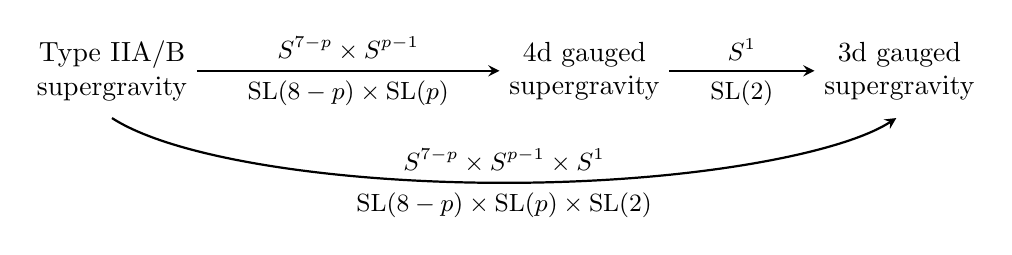
\begin{tikzpicture}
    \draw (0,0) node (10d) [align=center] {Type IIA/B \\ supergravity};
    \draw ($(10d)+(6,0)$) node (4d) [align=center] {4d gauged \\ supergravity};
    \draw ($(4d)+(4,0)$) node (3d) [align=center] {3d gauged \\ supergravity};

    \draw [thick, -stealth] (10d) -- (4d) node [midway, above] {\small $S^{7-p}\times S^{p-1}$} node [midway, below] {\small $\SL(8-p)\times \SL(p)$};
    \draw [thick, -stealth] (4d) -- (3d) node [midway, above] {\small $S^{1}$} node [midway, below] {\small $\SL(2)$};
    \draw [thick, -stealth] ($(10d)-(0,0.6)$) arc [start angle=-160,end angle=-20,x radius=5.3,y radius=1.25] node [midway, above] {\small $S^{7-p}\times S^{p-1}\times S^{1}$} node [midway, below] {\small $\SL(8-p)\times \SL(p)\times \SL(2)$};
    \end{tikzpicture}
  \end{aligned}
\end{equation}
The truncation from 10d to 3d is constructed using $\E_{8(8)}$ exceptional field theory, with isometries embedded as $\SL(8-p)\times\SL(p)\times\SL(2) \subset \E_{7(7)} \times \SL(2) \subset \E_{8(8)}$. Under $\E_{8(8)}\rightarrow\E_{7(7)}\times\SL(2)$, the ExFT coordinates decompose as
\begin{equation}
  \bm{248} \longrightarrow (\bm{1},\bm{3}) \oplus (\bm{56},\bm{2}) \oplus (\bm{133},\bm{3}).
\end{equation}
The $\E_{7(7)}$ coordinates sit in $(\bm{56},\bm{2})$. \ce{Further review ref.~\cite{Inverso:2016eet}? At least coordinates and cie. Details of IIA and IIB embeddings of forms?}

  \subsection{\texorpdfstring{$S^{3}\times S^{3}\times S^{1}$}{S3xS3xS1}}
  In ref.~\cite{Inverso:2016eet}, a truncation from type IIB to 4d on $S^{3}\times S^{3}\times S^{1}$ has been constructed. The type IIB two-forms $\hat{C}^{\alpha}_{\hat{\mu}\hat{\nu}}$ ($\alpha$ denotes a $\SL(2)_{\rm IIB}$ doublet) lead to seven-form field-strengths $H_{(7)}^{\alpha}=\d C_{(6)}^{\alpha}$. We search for singlets within $H_{(7)}^{\alpha}$ on $S^{3}\times S^{3}\times S^{1}$. Coordinates $\{y^{m}\}$ on $S^{3}\times S^{3}$, $z$ on $S^{1}$. Choice of gauge such that $H_{(7)}^{\alpha}$ given by
  \begin{equation}
    \partial_{z}C_{mnpqrs}^{\alpha}.
  \end{equation}
  Thus, we have to search for singlets in $C_{(6)}^{\alpha}$, built on $S^{3}\times S^{3}$ only. \ce{Is the choice of gauge always possible?}

  We first have to identify how $\SL(2)_{\rm IIB}$ is embedded in $\E_{7(7)}$ (which will help us to identify $\SL(2)_{\rm IIB}$ doublets like $C_{(6)}^{\alpha}$). To do so, we first follow ref.~\cite{Inverso:2016eet}, where the internal coordinates $\{y^{m}\}$ are embedded into $\E_{7(7)}$ following the decomposition $\E_{7(7)}\longrightarrow\SL(6)\times\SL(2)_{\rm IIB}\times\R^{+}_{\rm IIB}$:
  \begin{equation}
    \bm{56} \rightarrow (\bm{6'},\bm{1})_{-4} \oplus (\bm{6},\bm{2})_{-2} \oplus (\bm{20},\bm{1})_{0} \oplus (\bm{6'},\bm{2})_{2} \oplus (\bm{6},\bm{1})_{4},
  \end{equation}
  with coordinates in $(\bm{6'},\bm{1})_{-4}$. To build the truncation on $S^{3}\times S^{3}$, we are rather interested in the decomposition under $\E_{7(7)}\longrightarrow\SL(4)_{1}\times\SL(4)_{2}\times\R^{+}_{\SL(8)}$ (through $\SL(8)$):
  \begin{equation}
    \bm{56} \rightarrow \left[(\bm{6},\bm{1})_{2} \oplus (\bm{4},\bm{4})_{0} \oplus (\bm{1},\bm{6})_{-2}\right] \oplus \left[(\bm{1},\bm{6})_{2} \oplus (\bm{\bar{4}},\bm{\bar{4}})_{0} \oplus (\bm{6},\bm{1})_{-2}\right].
  \end{equation}
  We compare these two decompositions by further decomposing under
  \begin{equation}
    \begin{aligned}
     (i):&\qquad \E_{7(7)}\longrightarrow\SL(6)\times\SL(2)_{\rm IIB}\times\R^{+}_{\rm IIB} \longrightarrow \SL(3)_{1}\times\SL(3)_{2}\times\R^{+}_{\SL(6)}\times\R^{+}_{\SL(2)_{\rm IIB}}\times\R^{+}_{\rm IIB},\\
     (ii):&\qquad \E_{7(7)}\longrightarrow\SL(4)_{1}\times\SL(4)_{2}\times\R^{+}_{\SL(8)} \longrightarrow \SL(3)_{1}\times\SL(3)_{2}\times\R^{+}_{1}\times\R^{+}_{2}\times\R^{+}_{\SL(8)}.
    \end{aligned}
  \end{equation}
  We get the following:
  \begin{equation}
    \begin{aligned}
    \bm{56} &\overset{(i)}{\longrightarrow} \Big[(\bm{\bar{3}},\bm{1})_{-1,0,-4} \oplus (\bm{1},\bm{\bar{3}})_{1,0,-4}\Big] \oplus \Big[(\bm{3},\bm{1})_{1,1,-2} \oplus (\bm{3},\bm{1})_{1,-1,-2} \oplus (\bm{1},\bm{3})_{-1,1,-2} \oplus (\bm{1},\bm{3})_{-1,-1,-2}\Big] \\
    &\qquad \oplus \Big[(\bm{1},\bm{1})_{3,0,0} \oplus (\bm{1},\bm{1})_{-3,0,0} \oplus (\bm{3},\bm{\bar{3}})_{-1,0,0} \oplus (\bm{\bar{3}},\bm{3})_{1,0,0}\Big] \\
    &\qquad \oplus \Big[(\bm{\bar{3}},\bm{1})_{-1,1,2} \oplus (\bm{\bar{3}},\bm{1})_{-1,-1,2} \oplus (\bm{1},\bm{\bar{3}})_{1,1,2} \oplus (\bm{1},\bm{\bar{3}})_{1,-1,2}\Big] \oplus \Big[(\bm{3},\bm{1})_{1,0,4} \oplus (\bm{1},\bm{3})_{-1,0,4}\Big],\\[10pt]
    \bm{56} &\overset{(ii)}{\longrightarrow} \Big[(\bm{\bar{3}},\bm{1})_{2,0,2} \oplus (\bm{3},\bm{1})_{-2,0,2} \oplus (\bm{1},\bm{1})_{-3,-3,0} \oplus (\bm{1},\bm{3})_{-3,1,0}\oplus (\bm{3},\bm{1})_{1,-3,0} \oplus (\bm{3},\bm{3})_{1,1,0}\\
      &\quad\qquad \oplus (\bm{1},\bm{\bar{3}})_{0,2,-2} \oplus (\bm{1},\bm{3})_{0,-2,-2}\Big] \oplus \Big[(\bm{1},\bm{\bar{3}})_{0,2,2} \oplus (\bm{1},\bm{3})_{0,-2,2} \oplus (\bm{1},\bm{1})_{3,3,0} \oplus (\bm{1},\bm{\bar{3}})_{3,-1,0}\\
      &\quad\qquad \oplus (\bm{\bar{3}},\bm{1})_{-1,3,0} \oplus (\bm{\bar{3}},\bm{\bar{3}})_{-1,-1,0} \oplus (\bm{\bar{3}},\bm{1})_{2,0,-2} \oplus (\bm{3},\bm{1})_{-2,0,-2}\Big].
    \end{aligned}
  \end{equation}

  From these decompositions we extract the relations between the charges:
  \begin{equation}
    \begin{cases}
    q_{\SL(6)} = -\dfrac{1}{2}(q_{\SL(3)_{1}}+q_{\SL(3)_{2}}), \\[7pt]
    q_{\SL(2)_{\rm IIB}} = \dfrac{1}{4}\,\left(q_{\SL(3)_{1}}-q_{\SL(3)_{2}}+q_{\SL(8)}\right), \\[7pt]
    q_{\rm IIB} = \dfrac{1}{2}\,\left(-q_{\SL(3)_{1}}+q_{\SL(3)_{2}}+3\,q_{\SL(8)}\right).
    \end{cases}
  \end{equation}
  So the coordinates are inside $(\bm{6},\bm{1})_{-2}\oplus(\bm{1},\bm{6})_{2}$ of $\SL(4)_{1}\times\SL(4)_{2}\times\R^{+}_{\SL(8)}$. \ce{Problem with $3, \bar{3}$? Comes from identification $\bm{6'}=\bm{\bar{6}}$?}

  We now turn to the six-form potential $C_{(6)}^{\alpha}$, which sits in the representation $\bm{133}$ of $\E_{7(7)}$. Under $\E_{7(7)} \rightarrow \SL(8)$, it decomposes as $\bm{133} \rightarrow \bm{63} \oplus \bm{70}$, and
  \begin{equation}
    \begin{aligned}
    \SL(8) & \longrightarrow \SL(4) \times \SL(4) \times \R^{+} \\
    \bm{63} & \longrightarrow (\bm{4},\bm{\bar{4}})_{2} \oplus (\bm{1},\bm{1})_{0} \oplus (\bm{1},\bm{15})_{0} \oplus (\bm{15},\bm{1})_{0} \oplus (\bm{\bar{4}},\bm{4})_{-2} \\
    \bm{70} & \longrightarrow (\bm{1},\bm{1})_{4} \oplus (\bm{\bar{4}},\bm{4})_{2} \oplus (\bm{6},\bm{6})_{0} \oplus (\bm{4},\bm{\bar{4}})_{-2} \oplus (\bm{1},\bm{1})_{-4}.
    \end{aligned}
  \end{equation}
  Given that $C_{(6)}^{\alpha}$ is a $\SL(2)_{\rm IIB}$ doublet of fixed $R_{\rm IIB}^{+}$ charge, let us spell out the charges explicitly. In $\bm{63}$:
  \begin{equation}
    \begin{aligned}
    \SL(4) \times \SL(4) \times \R^{+} & \longrightarrow \SL(3) \times \SL(3) \times \R^{+}_{\SL(2)_{\rm IIB}} \times \R^{+}_{\rm IIB} \\
    (\bm{4},\bm{\bar{4}})_{2} & \longrightarrow (\bm{1},\bm{1})_{-1,6} \oplus (\bm{1},\bm{\bar{3}})_{0,4} \oplus (\bm{3},\bm{1})_{0,4} \oplus (\bm{3},\bm{\bar{3}})_{1,2}\\
    (\bm{1},\bm{1})_{0} & \longrightarrow (\bm{1},\bm{1})_{0,0} \\
    (\bm{1},\bm{15})_{0} & \longrightarrow (\bm{1},\bm{1})_{0,0} \oplus (\bm{1},\bm{3})_{-1,2} \oplus (\bm{1},\bm{\bar{3}})_{1,-2} \oplus (\bm{1},\bm{8})_{0,0}\\
    (\bm{15},\bm{1})_{0} & \longrightarrow (\bm{1},\bm{1})_{0,0} \oplus (\bm{3},\bm{1})_{1,-2} \oplus (\bm{\bar{3}},\bm{1})_{-1,2} \oplus (\bm{8},\bm{1})_{0,0} \\
    (\bm{\bar{4}},\bm{4})_{-2} & \longrightarrow (\bm{1},\bm{1})_{1,-6} \oplus (\bm{1},\bm{3})_{0,-4} \oplus (\bm{\bar{3}},\bm{1})_{0,-4} \oplus (\bm{\bar{3}},\bm{3})_{-1,-2}.
    \end{aligned}
  \end{equation}
  In $\bm{70}$:
  \begin{equation}
    \begin{aligned}
    \SL(4) \times \SL(4) \times \R^{+} & \longrightarrow \SL(3) \times \SL(3) \times \R^{+}_{\SL(2)_{\rm IIB}} \times \R^{+}_{\rm IIB} \\
    (\bm{1},\bm{1})_{4} & \longrightarrow (\bm{1},\bm{1})_{1,6}\\
    (\bm{\bar{4}},\bm{4})_{2} & \longrightarrow (\bm{1},\bm{1})_{2,0} \oplus (\bm{1},\bm{3})_{1,2} \oplus (\bm{\bar{3}},\bm{1})_{1,2} \oplus (\bm{\bar{3}},\bm{3})_{0,4} \\
    (\bm{6},\bm{6})_{0} & \longrightarrow (\bm{3},\bm{3})_{0,0} \oplus (\bm{3},\bm{\bar{3}})_{-1,2} \oplus (\bm{\bar{3}},\bm{3})_{1,-2} \oplus (\bm{\bar{3}},\bm{\bar{3}})_{0,0} \\
    (\bm{4},\bm{\bar{4}})_{-2} & \longrightarrow (\bm{1},\bm{1})_{-2,0} \oplus (\bm{1},\bm{\bar{3}})_{-1,-2} \oplus (\bm{3},\bm{1})_{-1,-2} \oplus (\bm{3},\bm{\bar{3}})_{0,-4} \\
    (\bm{1},\bm{1})_{-4} & \longrightarrow (\bm{1},\bm{1})_{-1,-6}
    \end{aligned}
  \end{equation}
  $\SO(3)\times\SO(3)$ singlets $\SL(2)_{\rm IIB}$ doublets and of given $R_{\rm IIB}^{+}$ charge are given by
  \begin{equation}
    (\bm{1},\bm{1})_{1,6} \oplus (\bm{1},\bm{1})_{-1,6} \subset (\bm{1},\bm{1})_{4} \oplus (\bm{4}, \bm{\bar{4}})_{2} \quad {\rm and} \quad (\bm{1},\bm{1})_{1,-6} \oplus (\bm{1},\bm{1})_{-1,-6} \subset (\bm{1},\bm{1})_{-4} \oplus (\bm{\bar{4}}, \bm{4})_{-2},
  \end{equation}
  where we wrote embeddings of $\SL(3) \times \SL(3) \times \R^{+}_{\SL(2)_{\rm IIB}} \times \R^{+}_{\rm IIB}$ in $\SL(4) \times \SL(4) \times \R^{+}$. These doublets correspond to $C_{(6)}^{\alpha}$ and the analogous $C^{(6)\,\alpha}$. So
  \begin{equation}
    C_{(6)}^{\alpha} \subset (\bm{1},\bm{1})_{4} \oplus (\bm{4},\bm{\bar{4}})_{2}.
  \end{equation}
  \ce{But no $(\bm{4},\bm{\bar{4}})$ in $\left((\bm{6},\bm{1})_{2}\oplus(\bm{1},\bm{6})_{-2}\right)^{\wedge 6}$...}

  \subsection{\texorpdfstring{$S^{7-p}\times S^{p-1}$}{S7-pxSp-1}}
  ...


\section{\texorpdfstring{${\rm AdS}_{3}\times S^{3}\times S^{3}\times S^{1}$}{AdS3xS3xS3xS1}}
Ten-dimensional maximal supergravity features a solution on ${\rm AdS}_{3}\times S^{3}_{+}\times S^{3}_{-}\times S^{1}$, whose vacuum preserves ${\cal N}=(4,4)$ supersymmetries. The superisometries are given by
\begin{equation}
  D^{1}(2,1;\alpha)_{\rm L}\times D^{1}(2,1;\alpha)_{\rm R},   
\end{equation}
with $\alpha$ the ratio of the spheres $S^{3}$ radii. The even part of $D^{1}(2,1;\alpha)$ is isomorphic to $\SL(2,\mathbb{R})\times\SO(3)^{+}\times\SO(3)^{-}$~\cite{Gunaydin:1986fe}, so that the bosonic symmetries at the vacuum are given by
\begin{equation}
  \underbrace{\SL(2,\mathbb{R})_{\rm L}\times\SL(2,\mathbb{R})_{\rm R}}_{\textstyle {\rm AdS}_{3}}\underbrace{\times\SO(3)^{+}_{\rm L}\times\SO(3)^{+}_{\rm R}}_{\textstyle S^{3}_{+}}\times\underbrace{\SO(3)^{-}_{\rm L}\times\SO(3)^{-}_{\rm R}}_{\textstyle S^{3}_{-}}.
\end{equation}

This vacuum has been described with an $\SO(8,8)$ embedding tensor $\theta_{IJ\vert KL}$ in ref.~\cite{Eloy:2020uix}. Possible to build an $\E_{8(8)}$ embedding tensor using $\theta_{IJ\vert KL}$~\cite{Deger:2019tem}: the maximal theory can be truncated to a half-maximal subsector upon truncating the coset space
\begin{equation} \label{eq:E8SO88}
{\rm E}_{8(8)}/{\rm SO}(16) \longrightarrow \SO(8,8)/(\SO(8)\times\SO(8)).
\end{equation}
Specifically, splitting the ${\rm E}_{8(8)}$ generators according to
\begin{equation}
  \left\{L^{[IJ]}, Y^{A}\right\},\quad I\in\llbracket1,16\rrbracket,\;\; A\in\llbracket1,128\rrbracket,
\end{equation}
into $\SO(8,8)$ and its orthogonal complement (transforming in the spinor representation ${\bf 128}_{\rm s}$ of $\SO(8,8)$), an embedding tensor of the maximal theory takes the form
\begin{equation} \label{eq:embmax}
  \begin{cases}
  \Theta_{IJ|KL} = \theta_{IJ|KL},\medskip\\
  \Theta_{A|B} =-\dfrac{1}{2}\theta\,\eta_{AB}+\dfrac{1}{96}\,\Gamma^{IJKL}_{AB}\,\theta_{IJ\vert KL},
  \end{cases}
\end{equation}
where $\Gamma^{IJKL}_{AB}$ denotes the four-fold product of $\SO(8,8)$ $\Gamma$ matrices. Spectrum computed in ref.~\cite{Eberhardt:2017fsi}, organized into long multiplets $\left[\ell^{+}_{R},\ell^{-}_{R},\ell^{+}_{L},\ell^{-}_{L}\right]$ of $D^{1}(2,1;\alpha)_{\rm L}\times D^{1}(2,1;\alpha)_{\rm R}$.

  \subsection{Deformations from \texorpdfstring{${\rm AdS}_{3}\times S^{3}$}{AdS3xS3}}
  In ref.~\cite{Eloy:2021fhc}, deformation of ${\rm AdS}_{3}\times S^{3}$ built from a $\SO(8,4)$ coset-representative $v(\omega,\zeta)$. For generic $(\omega,\zeta)$, ${\cal N}=0$, but along
  \begin{equation}
    \zeta^{2}=1-e^{-2\omega},
  \end{equation}
  ${\cal N}=(4,0)$.

  From this deformation, we can generate of deformation of ${\rm AdS}_{3}\times S^{3}_{+}\times S^{3}_{-}\times S^{1}$: first embed $v$ in ${\cal V}\in\SO(8,8)$, then deform embedding tensor $T={\cal V}^{-1}\cdot\theta$, and embed $T$ in $\E_{8(8)}$. Two different ways of embedding $v$ in $\SO(8,8)$ $\implies$ ${\cal V}^{(+)}(\omega_{+},\zeta_{+})$ and ${\cal V}^{(-)}(\omega_{-},\zeta_{-})$. Then, four-parameter deformation from
  \begin{equation}
    {\cal V}(\omega_{+},\zeta_{+},\omega_{-},\zeta_{-})={\cal V}^{(+)}{\cal V}^{(-)}.
  \end{equation}
  \ce{More possibilities?}

  Symmetries:
  \begin{equation}
   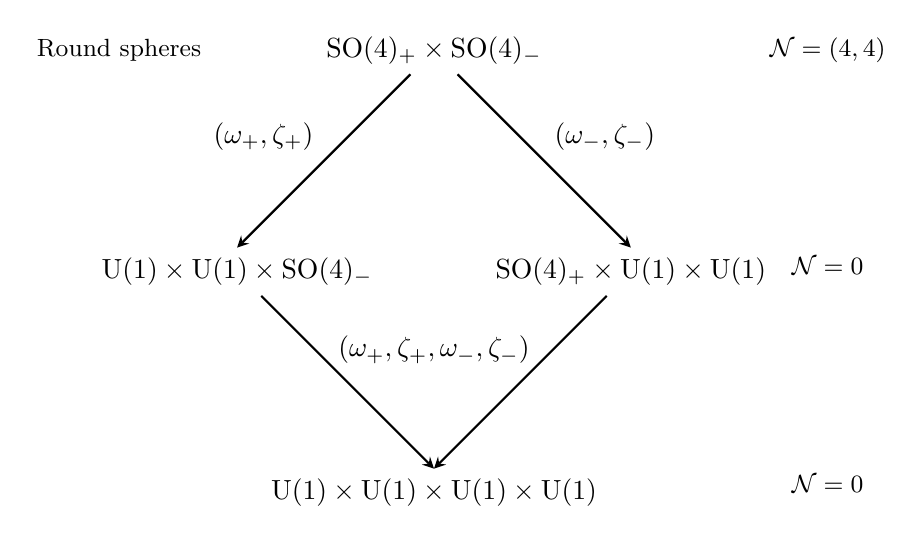
\begin{tikzpicture}
      \draw (0,0) node (round) {${\rm SO}(4)_{+} \times{\rm SO}(4)_{-} $};
      \draw ($(round)+(-4,0)$) node {\small Round spheres};
      \draw ($(round)+(5,0)$) node (susy) {\small ${\cal N}=(4,4)$};
      \draw [thick,-stealth] (round) -- +(-2.5,-2.5) node (defp) [below] {${\rm U}(1)\times{\rm U}(1) \times{\rm SO}(4)_{-}$} node [midway,above left] {$(\omega_{+},\zeta_ {+})$};
      \draw [thick,-stealth] (round) -- +(2.5,-2.5) node (defm) [below] {${\rm SO}(4)_{+} \times{\rm U}(1)\times{\rm U}(1)$} node [midway,above right] {$(\omega_{-},\zeta_ {-})$};
      \draw ($(susy)+(0,-2.5)$) node [below] {\small ${\cal N}=0$};
      \draw [thick,-stealth] (defm) -- +(-2.5,-2.5) node (defpm) [below] {${\rm U}(1)\times{\rm U}(1) \times{\rm U}(1)\times{\rm U}(1)$} node [above=1.2cm] {$(\omega_{+},\zeta_ {+},\omega_{-},\zeta_ {-})$};
      \draw [thick,-stealth] (defp) -- +(2.5,-2.5);
      \draw ($(susy)+(0,-5.5)$) node {\small ${\cal N}=0$};
    \end{tikzpicture}
  \end{equation}
  Two lines along which ${\cal N}=(4,0)$;
  \begin{equation}
    \begin{cases}
      \zeta^{2}_{+}=1-e^{-2\omega_{+}},\\
      \omega_{-}=\zeta_{-}=0,
    \end{cases}
    \quad 
    \begin{cases}
      \omega_{+}=\zeta_{+}=0,\\
      \zeta^{2}_{-}=1-e^{-2\omega_{-}}.
    \end{cases}
  \end{equation}
  \ce{More?}

  \subsubsection{Deformation \texorpdfstring{${\cal V}^{(+)}$}{V+}}
  Study of deformation with ${\cal V}^{(+)}$ with half-maximal theory (access to full spectrum). For $\zeta^{2}_{+}=1-e^{-2\omega_{+}}$, $D^{1}(2,1;\alpha)_{\rm L}$ broken, for even part:
  \begin{equation}
    \SL(2,\mathbb{R})_{\rm L}\times\SO(3)^{+}_{\rm L}\times\SO(3)^{-}_{\rm L} \longrightarrow \SL(2,\mathbb{R})_{\rm L}\times\SO(2)^{+}_{\rm L}\times\SO(3)^{-}_{\rm L}
  \end{equation}
  Then spectrum organized in terms of lon multiplet of $D^{1}(2,1;\alpha)_{\rm R}$, charge $q_{\rm L}^{+}$ and spin $j_{\rm L}^{+}$:
  \begin{equation}
    \left[\ell^{+}_{R},\ell^{-}_{R}\right]^{j_{\rm L}^{+}}_{_{\rm L}^{+}},
  \end{equation}
  with conformal weight:
  \begin{equation}
    \Delta_{q}^{\ell^{+},\ell^{-}} = -\frac{1}{2} + \frac{1}{2}\sqrt{1+\frac{4\ell^{+}(\ell^{+}+1)+q^{2}(e^{2\omega}-1)+4\alpha^{2}\ell^{-}(\ell^{-}+1)}{1+\alpha^{2}}}.
  \end{equation}
  For ${\cal V}^{(-)}$, $\alpha\rightarrow\alpha^{-1}$.

\appendix

\section{Miniminal ${\cal N}=(1,0)$ six-dimensional supergravity}
We consider reductions within the minimal ${\cal N}=(1,0)$ six-dimensional supergravity, leading to duality group $\SO(4,4)$ in three dimensions, from which the half-maximal cases ${\cal N}=(1,1)$ and ${\cal N}=(2,0)$ can be deduced (in those cases the duality group in three dimensions in $\SO(8,4)$).

The coordinates $X^{[MN]}$ of the $\SO(p,q)$ exceptional field theory of ref.~\cite{Hohm:2017wtr} sit in the adjoint $\bm{28}$ of $\SO(4,4)$. Under $\SO(4,4)\rightarrow\SO(3,3)\times\R_{+}$, it decomposes into
\begin{equation}  
  \begin{aligned}
    \bm{28} &\longrightarrow \bm{6}_{2} \oplus \bm{1}_{0} \oplus \bm{15}_{0} \oplus \bm{6}_{-2},\\
    X^{MN} &\longrightarrow \{Y^{A0},Y^{0}{}_{0},Y^{[AB]},Y^{A}{}_{0}\}.
  \end{aligned}
\end{equation}
Further decomposing $\SO(4,4)\rightarrow\SO(3,3)\times\R_{+}\rightarrow\SL(3)\times\R_{+}\times\R_{+}$, we get
\begin{equation}  \label{eq:decomp28SO8}
  \bm{28} \longrightarrow \left[\bm{\bar{3}}_{2,2} \oplus \bm{3}_{-2,2}\right] \oplus \bm{1}_{0,0} \oplus \left[\bm{3}_{4,0} \oplus \bm{1}_{0,0} \oplus \bm{8}_{0,0} \oplus \bm{\bar{3}}_{-4,0}\right] \oplus \left[\bm{\bar{3}}_{2,-2} \oplus \bm{3}_{-2,-2}\right].
\end{equation}
They are two physically different possibilities to embed the internal coordinates in $X^{MN}$, corresponding to the two different half-maximal supergravities in six dimensions:\footnote{The choices are equivalent in $\SO(4,4)$ (through triality), but different once embedded in $\SO(8,4)$.}
\begin{equation}  \label{eq:coordSO8}
  \begin{aligned}
    {\cal N}=(1,1):&\qquad y^{m}=Y^{m0}\subset\bm{\bar{3}}_{2,2} \longleftarrow \bm{6}_{2},\\
    {\cal N}=(2,0):&\qquad \tilde{y}_{m}=\varepsilon_{mnp}Y^{np}\subset\bm{3}_{4,0}\longleftarrow\bm{15}_{0}.
  \end{aligned}
\end{equation}

\paragraph{6d origin of the three-forms} The ${\cal N}=(1,0)$ supergravity features a two-form $\hat{B}_{\hat\mu\hat\nu}$. Both $\hat{B}_{\hat\mu\hat\nu}$ and its dual lead to two-form potentials in 3d. Their three-form field strengths are dual to purely internal three-form field-strengths $H_{(3)}$ and $*H_{(3)}$, of two-form potentials $C_{(2)}^{1}$ and $C_{(2)}^{2}$.

\paragraph{\boldmath $C_{(2)}^{1}$ and $C_{(2)}^{2}$ in $\SO(3,3)\times\R_{+}$} Given the decomposition~\eqref{eq:decomp28SO8} and the coordinates~\eqref{eq:coordSO8}, the two forms sit in the following representations:
\begin{equation}
  \begin{aligned}
    {\cal N}=(1,1):&\qquad C^{1}_{(2)}\subset\bm{\bar{3}}_{-4,0} \longleftarrow\bm{15}_{0}\quad{\rm and}\quad C^{2}_{(2)}\subset\bm{3}_{4,0} \longleftarrow\bm{15}_{0},\\
    {\cal N}=(2,0):&\qquad C^{1}_{(2)}\subset\bm{3}_{-2,2} \longleftarrow\bm{6}_{2}\quad{\rm and}\quad C^{2}_{(2)}\subset\bm{\bar{3}}_{2,2} \longleftarrow\bm{6}_{2}.
  \end{aligned}
\end{equation}

\paragraph{\boldmath $H_{(3)}$ and $*H_{(3)}$ in $\SO(3,3)\times\R_{+}$}
\begin{equation}
  \begin{aligned}
    {\cal N}=(1,1):&\qquad H_{(3)},*H_{(3)} \subset\bm{6}_{2}\otimes\bm{15}_{0}=\bm{6}_{2}\oplus\bm{10}_{2}\oplus\bm{\bar{10}}_{2}\oplus\bm{64}_{2},\\
    {\cal N}=(2,0):&\qquad H_{(7)},*H_{(7)} \subset\bm{10}_{0}\otimes\bm{6}_{2}=\bm{6}_{2}\oplus\bm{10}_{2}\oplus\bm{\bar{10}}_{2}\oplus\bm{64}_{2},
  \end{aligned}
\end{equation}

\paragraph{\boldmath $H_{(3)}$ and $*H_{(3)}$ in the embedding tensor} The embedding tensor of the $\SO(4,4)$ exceptional theory has two different components: $\theta_{[MNPQ]}\subset\bm{35_{\rm s}}\oplus\bm{35_{\rm c}}$ and $\theta_{(MN)}\subset\bm{35_{\rm v}}$. It decomposes as follows under $\SO(4,4)\rightarrow\SO(3,3)\times\R_{+}$:
\begin{equation}
  \begin{aligned}
    \bm{35_{\rm v}} &\longrightarrow \bm{1}_{4} \oplus {\color{mydarkorange}\bm{6}_{2}} \oplus \bm{1}_{0} \oplus \bm{20'}_{0} \oplus \bm{6}_{-2} \oplus \bm{1}_{-4},\\
    \bm{35_{\rm s}} &\longrightarrow {\color{mydarkorange}\bm{10}_{2}} \oplus \bm{15}_{0}  \oplus \bm{\bar{10}}_{-2},\\
    \bm{35_{\rm c}} &\longrightarrow {\color{mydarkorange}\bm{\bar{10}}_{2}} \oplus \bm{15}_{0}  \oplus \bm{10}_{-2},
  \end{aligned}
\end{equation}
where the colored representations are those coming from the three-forms. Only $\bm{10}_{2}$ and $\bm{\bar{10}}_{2}$ feature $\SO(4)$ singlets. \ce{So no distinction between (1,1) and (2,0)? Because triality, or I made errors?} $\leq$

\bibliography{ref}


\end{document}